\Transcb{yellow}{blue}{De Neutrino-Gamma connectie}
\onecolumn
{\blue IceCube: Spoor met $E_{dep} \sim 24$ TeV gezien op 22-sep-2017 20:54:30.43 UTC}\\
$\rightarrow$ EHE alarm (IC170922A) uitgezonden ($\sim 4$ per jaar) 
\begin{center}
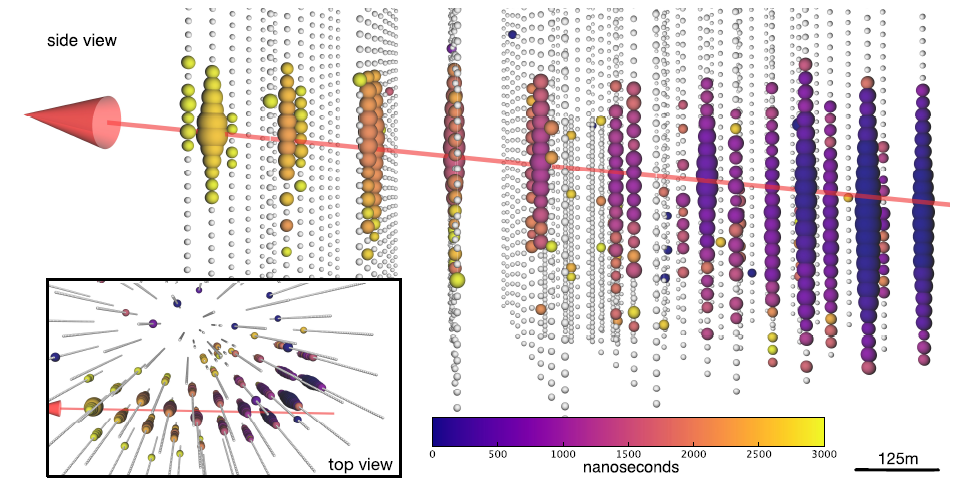
\includegraphics[keepaspectratio,height=12cm]{IC170922A-event}
\end{center}

\Tr
\onecolumn
IC170922A spoorparameters: $\alpha=77.43^{\circ +0.95}_{~-0.65} \quad \delta=5.72^{\circ +0.50}_{~-0.30} \quad E_{\nu}=290$ TeV
\begin{center}
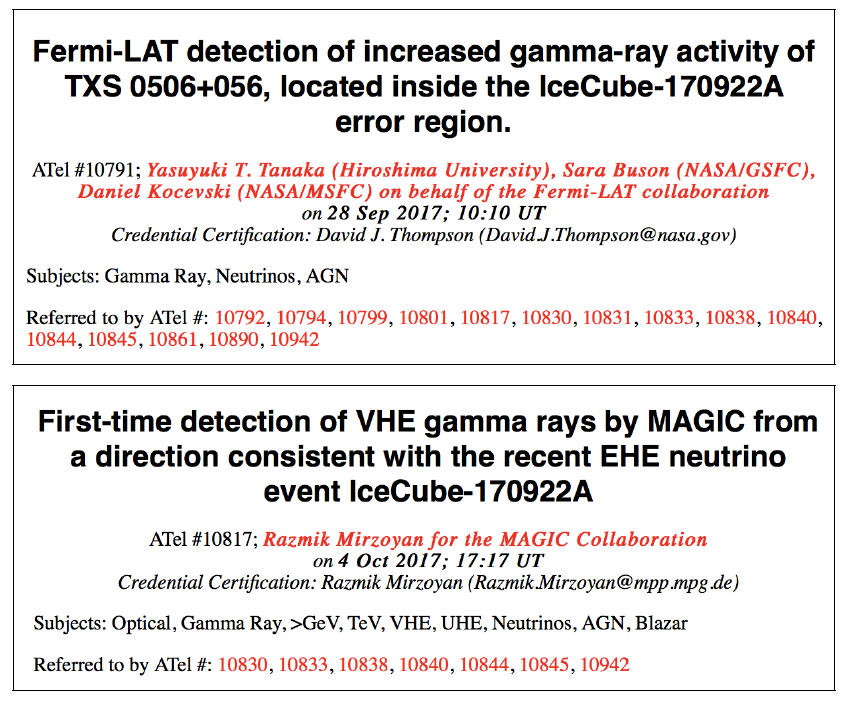
\includegraphics[keepaspectratio,height=14cm]{IC170922A}
\end{center}

\Tr
\onecolumn
\vspace*{2cm}
\begin{center}
{\blue Fermi lichtcurve voor IC170922A}\\[3mm]
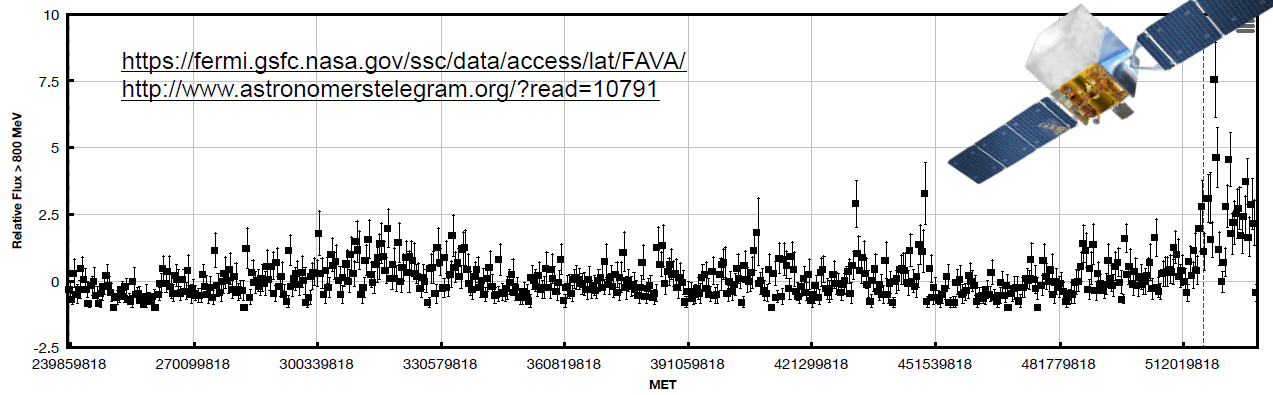
\includegraphics[keepaspectratio,width=25cm]{IC170922A-Fermi}
\end{center}

\Tr
\twocolumn[\begin{center}{\blue Het gebied rond IC170922A}\end{center}]
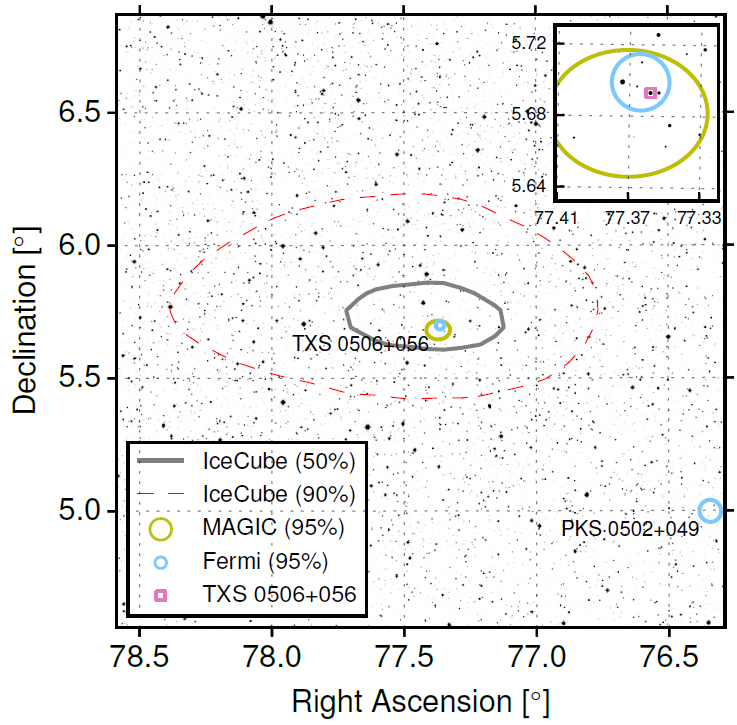
\includegraphics[keepaspectratio,width=13.5cm]{IC170922A-area}

\newpage

\begin{itemize}
\item Veel radio en X-ray bronnen
\item[] Meeste zijn erg zwak
\item 2 kandidaten blijven over\\
      {\large [Padovani et al. MNRAS 12-jul-2018]}
\item[$\ast$] TXS 0506+056 (Blazar $z=0.3365$)
\item[] $D_{phys}=1.37$Gpc ($\sim$4.5 Gly)
\item[$\ast$] PKS 0502+049 (FSRQ $z=0.954$)
\item[] $D_{phys}=3.29$Gpc ($\sim$11 Gly)
\item TXS valt samen met $\nu$ positie
\item[] PKS is $1.22^{\circ}$ verwijderd
\end{itemize}

\Tr
\onecolumn
\begin{center}
{\blue IceCube analyse op basis van archiefdata}
\end{center}
%
\begin{itemize}
\item Neem de TXS 0506+056 locatie als referentiepunt
\item[] $\rightarrow$ Zoek naar neutrino event clustering in positie en tijd
\item[] (elk event krijgt een gewicht op basis van energie en relatieve positie)
\end{itemize}
%
\begin{center}
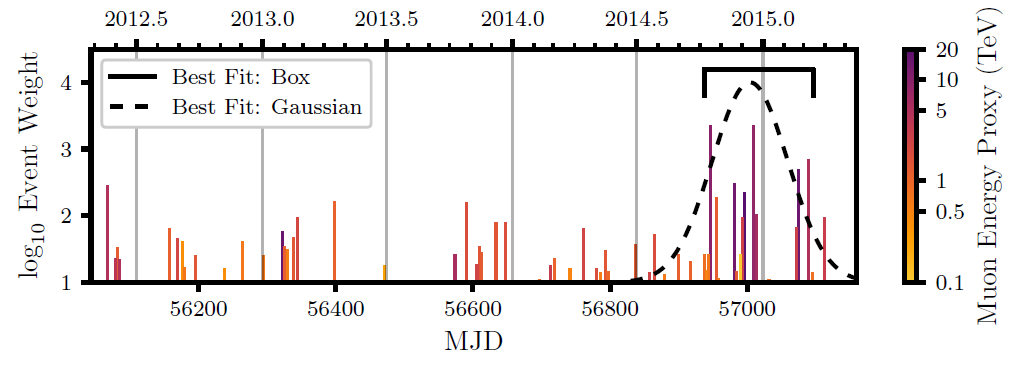
\includegraphics[keepaspectratio,width=24cm]{txs-time-dependent-IC86b}
\end{center}
%
\begin{itemize}
\item {\blue Neutrino activiteit rond 13-dec-2014 ($\pm$ 21 dagen) gedurende $110^{+35}_{-24}$dagen}
\end{itemize}
